\chapter*{ประวัติผู้เขียน}
\addcontentsline{toc}{chapter}{ประวัติผู้เขียน}

\vspace{0.2cm}

\noindent
\begin{minipage}[c]{0.28\textwidth}
    \centering
    \begin{tikzpicture}
        \fill[black!12] (0.04,-0.04) circle (1.4cm);
        \node[circle, draw=rbruGold, line width=2pt, inner sep=0pt] at (0,0) {
            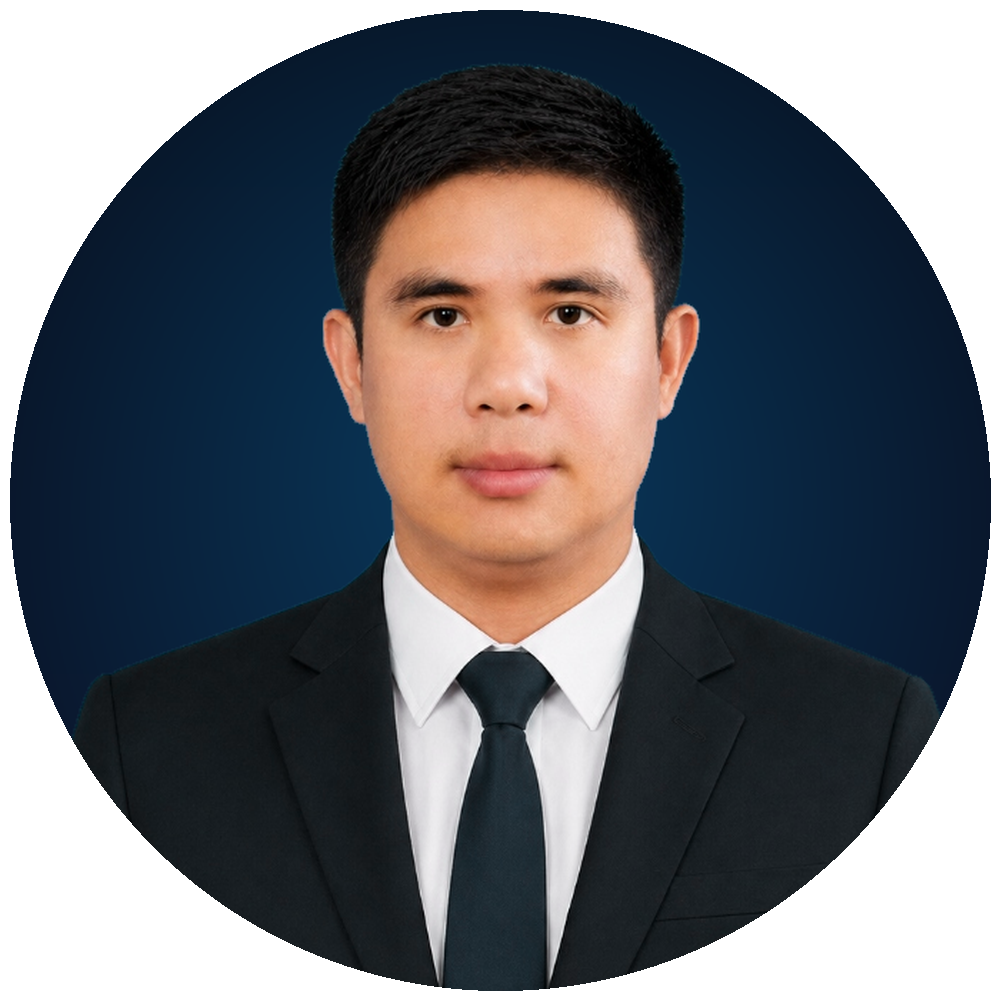
\includegraphics[width=2.7cm,height=2.7cm,keepaspectratio]{images/author_chewa_circle_final.png}
        };
    \end{tikzpicture}
\end{minipage}\hfill
\begin{minipage}[c]{0.69\textwidth}
    {\fontsize{16}{20}\selectfont\bfseries\color{rbruNavy} ผู้ช่วยศาสตราจารย์ ดร.ชีวะ ทัศนา}\\[0.2cm]
    {\fontsize{11.5}{16}\selectfont
    สาขาวิชาฟิสิกส์ คณะวิทยาศาสตร์และเทคโนโลยี\\
    มหาวิทยาลัยราชภัฏรำไพพรรณี\\[0.1cm]
    \textbf{อีเมล:} \texttt{chewa.t@rbru.ac.th}}
\end{minipage}

\vspace{0.4cm}
{\color{rbruSlate!30}\hrule height 0.8pt}
\vspace{0.4cm}

\noindent
\begin{minipage}[t]{0.48\textwidth}
    {\fontsize{13}{16}\selectfont\bfseries\color{rbruGreen} ประวัติการศึกษา}\par\vspace{4pt}
    \begin{itemize}\setlength{\itemsep}{2pt}\setlength{\parsep}{0pt}\setlength{\topsep}{2pt}\setlength{\partopsep}{0pt}\setlength{\leftmargin}{12pt}
        \item \textbf{ปร.ด. (ฟิสิกส์)} Ph.D. in Physics\\สาขาวิชาฟิสิกส์
        \item \textbf{วท.ม. (ฟิสิกส์)} M.Sc. in Physics\\สาขาวิชาฟิสิกส์
        \item \textbf{วท.บ. (ฟิสิกส์)} B.Sc. in Physics\\สาขาวิชาฟิสิกส์ (เกียรตินิยม)
    \end{itemize}

    \vspace{0.35cm}
    {\fontsize{13}{16}\selectfont\bfseries\color{rbruGreen} ภาระงานสอนประจำ}\par\vspace{4pt}
    \begin{itemize}\setlength{\itemsep}{2pt}\setlength{\parsep}{0pt}\setlength{\topsep}{2pt}\setlength{\partopsep}{0pt}\setlength{\leftmargin}{12pt}
        \item คณิตศาสตร์สำหรับฟิสิกส์ (Mathematics for Physics)
        \item ฟิสิกส์แผนใหม่ (Modern Physics)
        \item ปฏิบัติการฟิสิกส์ขั้นสูง (Advanced Physics Lab)
        \item ฟิสิกส์เชิงคำนวณ (Computational Physics)
    \end{itemize}
\end{minipage}\hfill
\begin{minipage}[t]{0.48\textwidth}
    {\fontsize{13}{16}\selectfont\bfseries\color{rbruGreen} ความเชี่ยวชาญและงานวิจัยที่สนใจ}\par\vspace{4pt}
    \begin{itemize}\setlength{\itemsep}{3pt}\setlength{\parsep}{0pt}\setlength{\topsep}{2pt}\setlength{\partopsep}{0pt}\setlength{\leftmargin}{12pt}
        \item ฟิสิกส์เชิงทฤษฎีและระเบียบวิธีทางคณิตศาสตร์ในฟิสิกส์ (Theoretical Physics \& Mathematical Methods)
        \item การจำลองปรากฏการณ์ทางฟิสิกส์ด้วยคอมพิวเตอร์และการคำนวณเชิงตัวเลข (Computational Physics)
        \item การประยุกต์ใช้เทคโนโลยีความจริงเสริมและความจริงขยาย (AR / VR / XR) ในการเรียนรู้วิทยาศาสตร์
        \item ปัญญาประดิษฐ์และวิทยาศาสตร์ข้อมูลเพื่อการศึกษา (AI in STEM Education)
    \end{itemize}
\end{minipage}
